\documentclass{article}

\usepackage{xcolor}
\usepackage[ruled]{algorithm2e}
%\usepackage{algorithmic}
\usepackage{amsmath}
\usepackage{amsfonts}
\usepackage{amsthm}
\usepackage{graphicx}
\newtheorem{theorem}{Theorem}
\newtheorem{cxampl}[theorem]{Counterexample}
\newtheorem{lemma}[theorem]{Lemma}

\newcommand{\TODO}[1]{\begingroup\color{red}#1\endgroup}
\newcommand{\NR}[1]{\begingroup\color{orange}#1\endgroup}
\newcommand{\PFS}[1]{\begingroup\color{green}#1\endgroup}


\begin{document}

\title{Phylogenetics with Mixing Hybrids}

\maketitle


\begin{abstract}
  super-cool abstract
\end{abstract}

\section{Introduction}

Classical phylogenetics assumes an underlying branching process that
occasionally generates novel species. 



\begin{itemize}
\item evolution of gene clusters as in~\cite{Prohaska:17a}
 \item evolutionary events considered where either duplication 
 or recombination events (since losses cannot be observed when 
 we there is only one species under consideration)
 \item recombination events can happen due to unequal crossing
 over during mitosis
 \item if the breakpoint is in a gene, the resulting gene is
 a recombinant of its two parent genes ($x$ and $y$) who are
 considered to be adjacent
 \item here: lifting adjacency constraint of ''recombination''
 \item application to languages: e.g. English lexicon is said
 to contain 29\% Latin and as well as 29\% French words that 
 did not derive from its Germanic root which only contributes 
 with 25\%~\cite{Finkenstaedt:73}.
\end{itemize}


\section{R-Metrics} 

\subsection{Definition} 

In~\cite{Prohaska:17a} we introduced R-metrics by means of a simple
iterative scheme starting from a pair of points $\{x,y\}$ with a given
distance $d_{xy}$.  First, an additional point $z$ is inserted as a
``mixture'' of two parents $x$ and $y$ with a mixture ratio $a$. We assume
that the distance of $d_{zu}$ correspondinly is a mixture of $d_{xu}$ and
$d_{yu}$. More precisely, we assume that
\begin{equation} 
\begin{split} 
  d_{zx} & = (1-\alpha)  d_{xy} \\
  d_{zy} & =   \alpha    d_{xy} \\
  d_{zu} & =   \alpha    d_{xu} + (1-\alpha)  d_{yu} \quad\textrm{for all}\ 
                     u\in V\setminus\{ x,y \}
\end{split}
\end{equation} 
Then all points diverge with arbitrary rates, i.e., 
\begin{equation} 
  d_{pq}' = d_{pq} + \delta_p + \delta_q \quad\textrm{for all}\ 
  p,q \in V\cup\{z\} 
\end{equation} 
We say that a metric distance $d$ is an R-metric if it can be constructed
in this manner. An iteration with $a\in(0,1)$ will be referred to as
\emph{merge step}, since the product $z$ is a mixture of the parents $x$
and $y$. If $a=1$ or $a=0$ we speak of a \emph{branch step} since
$z$ originates as a copy or $x$ or $y$, respectively. As noted in
\cite{Prohaska:17a}, every additive metric is an R-metric.

\subsection{R-metrics on 4 Points}

Every metric on three points $X=\{x,y,u\}$ is additive and can be written as
\begin{equation}
  d_{xy}=a+b \qquad
  d_{xu}=a+c \qquad
  d_{yu}=b+c\,. 
\end{equation}
By construction, every R-metric on four points thus arises by a single
split or hybridization step from a metric on three points. W.l.o.g.\ we
assume that $x$ and $y$ act as parents and obtain on $\{x,y,z,u\}$:
\begin{equation} 
  \begin{split}
  d_{xy}' & = a + b + \delta_x + \delta_y \\  
  d_{xz}' & = (1-\alpha)(a+b) + \delta_z +\delta_x \\
  d_{xu}' & = a + c + \delta_x + \delta_u \\
  d_{yz}' & = \alpha (a+b) + \delta_y + \delta_z \\
  d_{yu}' & = b + c + \delta_y + \delta_u \\
  d_{zu}' & = \alpha (a+c) + (1-\alpha)(b+c) + \delta_z + \delta_u
\end{split}
\end{equation}
On the other hand, every metric on 4 points is totally split decomposable
and has a unique represention as a ``box with spikes'' as shown in
Fig.~\ref{fig:4box}.

\begin{figure}
  \begin{center}
    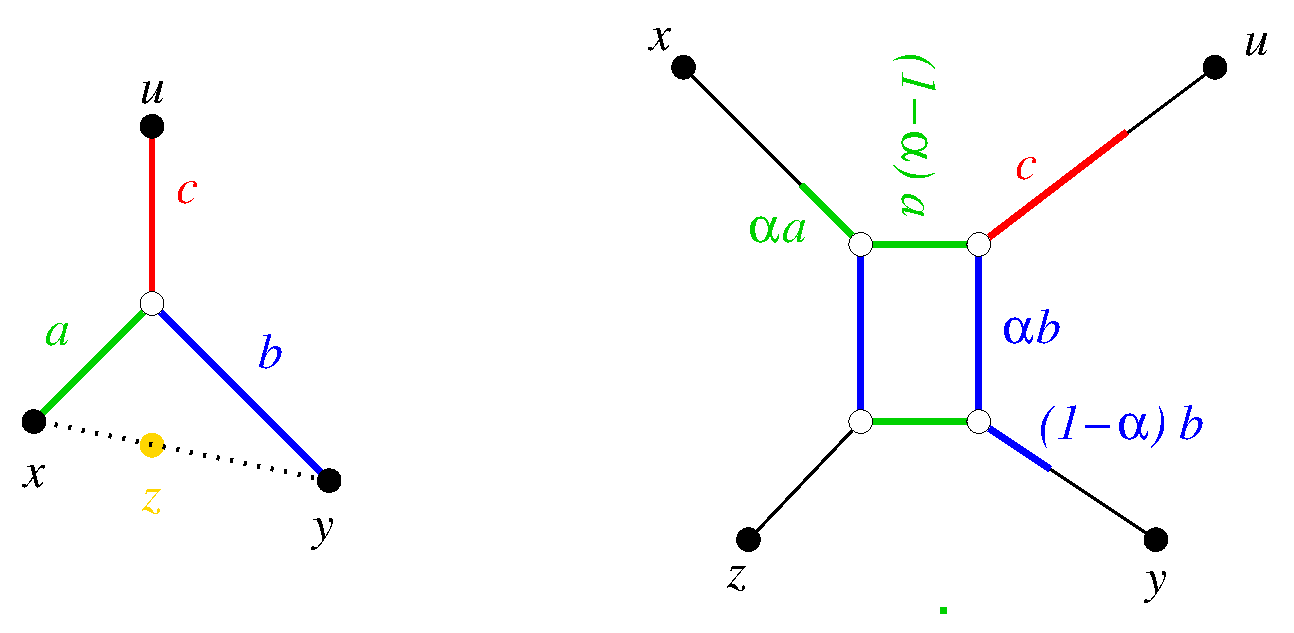
\includegraphics[width=0.75\textwidth]{n4.eps}
  \end{center}
  \caption{General form an R-metric on $\{x,y,z,u\}$ where $z$ arises by
    merging the parents $x$ and $y$.}
  \label{fig:4box}
\end{figure}

The isolation indices for the non-trivial splits are
obtained from the three distance sums
\begin{equation*}
  \begin{split}
    d_{xy}'+d_{zu}' & =  a + b + (1-\alpha)a + \alpha b + \xi \\
    d_{xz}'+d_{yu}' & = \alpha (a+b) + b + \xi \\
    d_{xu}'+d_{yz}' & = (1-\alpha)(a+b) + a + \xi \\
  \end{split}
\end{equation*}
where $\xi=\delta_x+\delta_y+\delta_z+\delta_u$. A short computation shows
\begin{equation*}
  \begin{split}
    (d_{xy}'+d_{zu}')-(d_{xz}'+d_{yu}') &= 2(1-\alpha)a \ge 0 \\
    (d_{xy}'+d_{zu}')-(d_{xu}'+d_{yz}') &= 2\alpha b \ge 0 \,,\\
  \end{split}
\end{equation*}
whence the non-trivial isolation indices are $\beta_{xz|yu}=(1-\alpha)a$
and $\beta_{yz|xu}=\alpha b$. The four trivial isolation indices are
\begin{equation*}
  \beta_{z|xyu} = \delta_z \qquad
  \beta_{u|xyz} = c + \delta_u \qquad
  \beta_{x|yzu} = \alpha a + \delta_x \qquad
  \beta_{y|xzu} = (1-\alpha) b + \delta_y 
\end{equation*}
We note, furthermore, that for $a,b>0$, both isolation indices are strictly
positive if and only if $0<\alpha<1$. For $\alpha=0$ we obtain the tree of
the form $(xz)(yu)$ and for $\alpha=1$ we the tree $(yz)(xu)$. In the
degenerate case in which either $a=0$ or $b=0$ the metric also reduces to a
tree. 

We are now in the position to characterize R-metrics in terms of its spiked
box diagram:
\begin{theorem}
  A metric on four points with non-trivial isolation isolation indices
  $r$ and $s$ is an R-metric if an only if there is pair of antipodal
  trivial splits with isolation indices $p$ and $q$ such that
  $p q \ge r s$. 
\end{theorem}
\begin{proof}
  Consider the diagram in Fig.~\ref{fig:4box}. Here, $z$ is a merge-child
  of $x$ and $y$ if and only if there is $\alpha\ge 0$ such that
  $p=:\beta_{x|yzu}\ge \alpha a$ and $q=:\beta_{y|xzu}\ge (1-\alpha
  b)$. Note that the other pair of antipodal spikes, i.e., $c+\delta_u\ge0$
  and $\delta_z\ge0$ can be chosen arbitrarily. If $r=0$ or $s=0$ the
  metric is additive and thus an R-metric. Hence it suffices to consider
  the case that $r,s>0$ and thus $0<\alpha<1$.

  The corresponding non-trivial isolation indices are
  $r:=\beta_{xz|yu}=(1-\alpha)a$ and $s:=\beta_{yz|xu}=\alpha b$, and thus
  $a=r/(1-\alpha)$ and $b=s/\alpha$. With the abbreviation
  $\zeta=\alpha/(1-\alpha)$, this implies $p\ge \zeta s$ and
  $q\ge (1/\zeta) r$, i.e., $p/s \ge \zeta \ge r/q$. A $\zeta>0$ satisfying
  these inequalities exists iff $p q \ge r s>0$. Since
  $\alpha = \zeta/(1+\zeta)$ we have $\alpha\in (0,1)$ for
  $\zeta\in(0,\infty)$.
\end{proof}

It follows immediately that the construction of R-metrics in four points is
not unique: In general both pairs of antipodal points may serve as as
parents. Furthermore, if $x,y$ are parents, then both $u$ and $z$ can be
obtained as child of a merge operation.


\TODO{maybe a closer look at the cases $a=0$ and $b=0$. This yields a tree
  in a very strange way!}




\subsection*{Other Stuff} 



As an immediate consequence we see that an R-metric whose construction
contains a merge step with $\alpha\in(0,1)$ cannot be additive. To see this
simply consider the 






Conversely, an
R-metric is additive if (and only if) all iterations are branching steps.








The iterative construction above contains an obvious source of ambiguity.
In every interation, a distance increment $\delta_u$ is added for all
points, including also the ones that are not involved in a branch or merge
event. Therefore several increments can be added to a point in consecutive
non-event iterations. It is clear that there is no way in which these
contributions can be disentangled: only their sum -- more precisely the sum
of $\delta_u$-value added between two consecutive events involving $u$ can
possibly be identified. Therefore we modify the construction rule such that
$\delta_u=0$ for all $u\in V\setminus\{x,y,z\}$. In addition we stipulate
$\delta_x=0$ for $a=0$ and $\delta_y=0$ for $a=1$, i.e., in branch events.

The iterative steps in this modified construction for R-metrics can be
encoded as an ordered list $\mathcal{S}$ of merge and branch
events together with the pertinent parameters: \\
\begin{itemize} 
\item[] A branch event is characterized by $[(x:z),\delta_x,\delta_z]$.
\item[] A merge event is characterized by
  $[(x,y:z),a,\delta_x,\delta_y,\delta_z]$.
\end{itemize}
For each event, $z$ is the offspring, while $x$ (and $y$) are the parent(s)
of the event. Note that each event has exactly one offspring. We call such
a list of events that explain $\mathcal{S}$ a \emph{scenario}.  Since every
metric on $|V|=3$ points is a additive and this described a tree, the first
event of $\mathcal{S}$ can always be represented as a branch event. It is
clear from the definition of R-metrics that every scenario $\mathcal{S}$
informs the recursions defining R-metrics and thus result in an R-metric.

\TODO{I think we also can uniquely resolve the temporal order of events:
  If $[x,y':z']$ predates $[x,y'':z'']$ in $\mathcal{S}$, then this
  temporal order must be maintained in all alternative scenarios.}

Given a scenario $\mathcal{S}$ we say that event $\alpha$ \emph{immediately
  pre-dates} event $\beta$, in symbols $\alpha \prec\beta$, if the
offspring of $\alpha$ is a parent of $\beta$. The relation $\prec$ defines
a directed acyclic graph, and thus a partial order on the set of events,
which we also denoted by $\prec$ from here on. This \emph{causal event
  partial order} $\prec$ can be understood as follows: $\alpha\prec\beta$
if and only if of the parents of $\beta$ is a descendant of $\alpha$. A key
observation is the following:
\begin{lemma}
  Every total order of a set events $\mathcal{S}$ consistent with the
  causal partial order $\prec$ yields the same R-metric.
\end{lemma}
\begin{proof}
  Obvious ... but maybe give a proof anyway ? 
\end{proof}















The definition of an R-matrix makes an important, and in practise
restrictive, assumption: For every merge event $(x,y:z)$ we assume that
there are surviving descendants of $x$, $y$, and $z$ that are not products
of a merge.

\TODO{As an open question for the future, we thus ask how an arbitrary 
submatrix of an R-metric can be recognized.} 

\subsection*{Properties of R-metrics} 




Conversely, it is not hard to construct examples of R-metrics that are not
split-decomposable.







\TODO{It does not seem to be very easy to check whether R-metric are 
totally decomposable or not. There is a reasonably easy 5-point condition
for that, however:

Set 
\begin{equation} 
  \alpha(tu|vw) := 
  \max\left\{ d_{tu}+d_{vw}, d_{tv}+d_{uw}, d_{tw}+d_{vu} \right\} -
             (d_{tu}+d_{vw})
\end{equation} 

Then Thm.6 of \cite{Bandelt:92} states that the metric is \emph{totally
  decomposable} iff and only if for all $t,u,v,w,x\in V$ holds 
\begin{equation} 
  \alpha(tu|vw) \le \alpha(tx|vw)+\alpha(tu|vx)
\end{equation} 

CAN YOU PLEASE CHECK THIS NUMBERICALLY as a first step. If we see that the 
R-metrics are totally decomposable in a large number of randomly generated
examples it will be worth while to show that analytically, presumably by 
proving that our construction the inequality above whenever.
}

\section{From Recognition to Approximation} 

\subsection{Recognition of R-metrics}

In \cite{Prohaska:17a} we showed that R-metrics can be recognized using
Alg.~\ref{alg:recogR} in $O(|V|^6)$ time.

We call the result $z$ of a merge event $(x,y:z)$ terminal this merging
step was not followed by another merge or branch event involving $z$. A
branch event $(x:z)$ is terminal if neither of its descendants was subject
to a further merge or branch event. It is clear that every R-metric
contains at least one merge or branch event. Alg.~\ref{alg:recogR}
\cite{Prohaska:17a} recognizes R-metrics $O(|V|^6)$ time. In each
interation it identifies a terminal merge or branch event and reduces the
problem by eliminating one of the two descendants of a branch event or the
mixed offspring of a merge event. It does not quite reconstruct the
individual interations faithfully since in the case of terminal branch
events $(x:z)$ no effort is made to precisely locate the common ancestor of
$x$ and $z$. As we shall see below, this can be done with moderate effort.
We also note that in the construction recipe a constant $\delta_u$ is added
in each to iteration to the branch of every point $u$, in particular also
those $u$ that are not involved in a merge or branch event. These
individual steps cannot be resolved: only the total increase in distance
between two merge or branch events can be resolved. Therefore, we set
$\delta_u=0$ for all $u$ not involved in an event. 

\begin{algorithm}[H]
\caption{Recognition of R-metrics}
\label{alg:recogR}
\SetAlgoLined

\While{$|V|>3$}{
  \For{$\{x,y,z\} \in V$}{
    \For{$\{u,v\} \in V\setminus\{x,y,z\}$}{
      $a_{u,v} := 
      \frac{(d'_{uz}+d'_{vy})-(d'_{vz}+d'_{uy})}{(d'_{ux}+d'_{vy})-(d'_{vx}+d'_{uy})}$\;
    }
    \If{$\forall a_{u,v}: a_{u,v}=a$ \,\&\, $a\in [0,1]$}{
      \If{$a \neq 0,1$}{
        \tcc{merge $(x,y:z)$} 
        $\delta_z = \frac{1}{2}(d'_{xz}+d'_{yz}-d'_{xy})$\;
        $d_{xy} = \frac{(d'_{uz}-a d'_{ux}-(1-a) d'_{uy})-
          2 \delta_z + a d'_{xz}+(1-a) d'_{yz}}{2a(1-a)}$\;
        $\delta_x = d'_{xz} - (1-a) d_{xy} - \delta_z$\;
        $\delta_y = d'_{yz} -   a   d_{xy} - \delta_z$\;
        $\forall u\in V\setminus\{x,y,z\}$ and $\forall p\in\{x,y\}$ set   
        $d_{up} = d_{pu} -\delta_p$\;
      }
      \tcc{If $a=1$ then split $(x:z)$} 
      \tcc{If $a=0$ then split $(y:z)$}
%      \TODO{why are the things above in a comment?} Because for
%      recognition only we don't do anything except dropping $z$
      $V\leftarrow V\setminus\{z\}$\;
      \textbf{continue}\;
    }  
  }
  \tcc{ no split or merge found for $\{x,y,z\}$ } 
  \Return \emph{\textbf{false}}
}
\Return \emph{\textbf{true}}
\end{algorithm}

\subsection{Extraction of Branch and Merge Scenarios} 

Our goal here is to modify Alg.~\ref{alg:recogR} into a consistent
approximation algorithm. More precisely, we set out to construct an
algorithm $\mathbb{A}$ with the following properties:
\begin{itemize} 
  \item For every finite metric $d$ on $|V|$ points, $\mathbb{A}(d)$ 
    is an R-metric
  \item If $d$ is a R-metric, then $\mathbb{A}(d)=d$.
\end{itemize} 
In practise the subdivide $\mathbb{A}$ into two steps: In the first stage,
we extract a scenario $\mathcal{S}$ of merge and branch events from $d$. In
the second stage, this scenario is converted back into a metric distance
$d(\mathcal{S})$.

The non-trivial part is the inference of a scenario $\mathcal{S}$ from an
arbitrary metric $d$ on $V$. Given a metric distance matrix $d$, we say
that a candidate event $(x,y:z)$ is \emph{perfect} if $a_{uv}$ as defined
in Alg.~\ref{alg:recogR} is the same for all $u,v\in V\setminus\{x,y,z\}$
and satisfied $a\in [0,1]$. If $a=1$ or $a=0$, we speak of perfect branch
candidate $(x:z)$ or $(y:z)$, if $0<a<1$, we speak of a perfect merge
candidate. The basic idea is now to iteratively identify candidates that
are as close to perfect as possible and to reduce the matrix by the best
branch or merge candidate. This overall logic is summarized in
Alg.\ref{alg:toplevel}.

\begin{algorithm}[H]
\caption{Consistent Approxmation of R-metrics}
\label{alg:toplevel}
\SetAlgoLined
\While{$|V|\ge 4$}{
  determine best branch step $(x:z)$\;
  determine best merge step $(x,y:z)$\;
  perform the best of split $(x:z)$ or merge $(x,y:z)$ step\;
  remove $z$ from and $V$\; 
}
compute initial branch scenario for $|V|\le 3$ leaves\;
\Return $\mathcal{S}$ 
\end{algorithm} 

Clearly, if $d$ is a R-metric, then there is always a perfect terminal
event that is recognized by Alg.\ref{alg:toplevel}, allowing a reduction of
the matrix by undoing the terminal merge or branch event and removing the
vertex $z$. Naturally, we obtain an approximation scheme that eventually
returns scenario $\mathcal{S}$ be settling for the best candidate in each
iteration step. As we shall see, some precautions have to be taken to
ensure that the scenario stays valid in the non-perfect case. More
importantly, it is not obvious what exactly the ``best candidate'' is
supposed to be. Before we address this issue in detail, we first describe
the reduction steps given that a candidate event has been selected in a
given iteration.

First we consider the special case of a branch steps. By Equ.(9) of
\cite{Prohaska:17a}, we have $a=0$ iff $d'_{uz}-d'_{vz} = d'_{uy}-d'_{vy}$
for all $y$ and $a=1$ iff $d'_{uz}-d'_{vz} = d'_{ux}-d'_{vx}$. These two
cases are effectively the same, identifying $x$ and $y$, respectively, as
the ancestral branch from which $z$ is split off. For the branch event
$(x:z)$ we obtain, by setting $a=1$, that $d'_{xz}=\delta_x+\delta_z$ and
$d'_{ux}-d'_{uz}=\delta_x-\delta_z$, whence
$d'_{xz}+d'_{ux}-d'_{uz}=2\delta_x$ and
$d'_{xz}+d'_{uz}-d'_{ux}=2\delta_y$. For numerical stability it seems
advisable to first compute the average
\begin{equation} 
  C := \frac{1}{|V|-2} \sum_{u\in V\setminus\{x,y\}} (d'_{ux}-d'_{uz})
\end{equation} 
in order to obtain the consensus values $\delta_x = (d'_{xz}+C)/2$ and
$\delta_z = (d'_{xz}-C)/2$.  We note, finally, there is no difference
whether $z$ as branching off from $x$ or \textit{vice versa}, hence it
suffices to consider only the $x$ small than $z$ in input order. 

\begin{algorithm}[H]
\caption{Branch($x:z$)} 
\label{alg:branchstep}
\SetAlgoLined
estimate consensus value for $C:=(d'_{ux}-d'_{uz})$ for $u\in
V\setminus\{x,z\}$ \;
$\delta_x = (d'_{xz}+C)/2$\;
$\delta_z = (d'_{xz}-C)/2$\;
$\forall u\in V\setminus\{x,z\}$: $d_{ux} =  d_{ux}-\delta_x$\;
\end{algorithm} 

For a merge step $(x,y:z)$ we essentially follow the reduction outline in
Alg.~\ref{alg:recogR}. As in the case of $\delta_x$ and $\delta_z$ in
Alg.~\ref{alg:branchstep} there a terms that can be obtained using
arbitrary choices of $u\in V\setminus\{x,y,z\}$. In particular that
pertains to the mixing parameter $a$, the value of $Q$, and the derived
quantity $d_{xy}$. For non-perfect candidates, it is desirable to estimate
robust average or consensus values instead of picking a particular value.
In Alg.~\ref{alg:mergestep} we us a simplistic scheme in which we assume
that a consensus value $\hat a$ for the mixture parameter to be supplied
already with the best candidate $(x,y:z)$. Given $\hat a$, it is most
natural to estimate $Q$ as an arithmetic mean. All other parameters are
then uniquely determined.

\begin{algorithm}[H]
\caption{Merge($x,y:z$)} 
\label{alg:mergestep} 
\SetAlgoLined
use $a$ estimated for $(x,y:z)$\;
$\delta_z = \frac{1}{2}(d'_{xz}+d'_{yz}-d'_{xy})$\;
estimate consensus value for $Q:=(d'_{uz}-a d'_{ux}-(1-a) d'_{uy})$ for the 
set $u\in V\setminus\{x,y,z\}$\;
$d_{xy} = (Q-2 \delta_z + a d'_{xz}+(1-a) d'_{yz})/(2a(1-a))$\;
$\delta_x = d'_{xz} - (1-a) d_{xy} - \delta_z$\;
$\delta_y = d'_{yz} -   a   d_{xy} - \delta_z$\;
$\forall u\in V\setminus\{x,y,z\}$ and $\forall p\in\{x,y\}$ set   
$d_{up} = d_{pu} -\delta_p$\;
repair metric if necessary\;
\end{algorithm} 

The incremental modifications in Alg.~\ref{alg:branchstep} and
\ref{alg:mergestep} are not guaranteed to preserve metrics. Furthermore,
several other inequalities must hold and may need be enforced. First,
$\delta_x,\delta_y,\delta_z\ge 0$, $d_{xy}\ge 0$, and $d_{ux},d_{uy}\ge
0$. In order to enforce the triangle inequality after the editing step, one
could use one of several \emph{triangle fixing} algorithms that have been
designed to find the metric closest to a given dissimilarity measure, see
e.g.\ \cite{Sra:05,Brickel:08}. Recently, algorithms have appeared that
restrict themselves to fixing only triangles that violate the triangle
inequality \cite{Gilbert:17}. For our purposes, Algorithm 2 of
\cite{Gilbert:17} seems particularly appropriate.

\subsection{Ranking of Branch and Merge Scenarios}

Let us now turn to the problem of finding best candidates. First suppose
there are perfect branch or merge candidates. In this case it seems
advisable to follow the logic of clustering algorithms and to consider the 
ones with smallest distances first. This choice does not influence the
correctness of the recognition algorithm but should contribute to numerical
stability.

If there is no perfect candidate, however, our choice will affect the final
result. Ideally, we would like to select a sequence of candidates that
minimizes the overall difference between the input and the output metric.
This seems to be difficult at the very least since in practise we have to
make a choice in each iteration step. Therefore we resort to heuristics
that at least guarantee that perfect candidates are recognized as such.

For the branch candidates, Algorithm~\ref{alg:branchstep} is a rather
straightforward choice. It obviously ensures that a perfect branch step,
i.e., one with $\epsilon_{xz}=0$, receives highest priority.

\begin{algorithm}[H]
\caption{Find best branch candidate $(x:z)$ } 
\label{alg:branchstep}
\SetAlgoLined
\For{$\{x,z\} \subseteq V$}{
  \For{$\{u,v\}\in V\setminus\{x,z\}$}{ 
    $\epsilon_{xz} += \Vert (d_{vz}-d_{uz})- (d_{vx}-d_{ux}) \Vert$\;
  }   
}
\Return ranked list $[(x:z,\epsilon_{xz})| x,z\in V]$ by increasing 
$\epsilon_{xz}$\;
\end{algorithm} 

For merge candidates, the problem is bit more involved. The quality $q_a$
of the merge candidate $(x,y:z)$ is determined by how tightly
$a=(h_z-h_y)/(h_x-h_y)$ is centered at a single value $\hat a\in (0,1)$ for
all $u,v\in V\setminus\{x,y,z\}$. Since there is nothing to prevent the
denominator $h_x-h_y$ from becoming $0$, estimating $\hat a$ is also a not
entirely trivial problem.

A short computation shows that $a\in(0,1)$ if and only if $h_z$ lies
between $h_x$ and $h_y$. Correspondingly, we have $a<0$ for $h_z>h_y>h_x$
or $h_z<h_y<h_x$ and $a>1$ for $h_z>h_x>h_y$ or $h_z<h_x<h_y$.  This
suggests a step-wise evaluation:
\begin{itemize} 
\item[(i)] determine for the $\{u,v\}\in V\setminus\{x,y,z\}$ to which of
  three categories the triple $(h_x,h_y,h_z)$ belongs. If it is one of the
  latter two cases, reject the merge step and $(x,y:z)$ treat as one of of
  the branch steps $(x:z)$ or $(y:z)$.
\item[(ii)] If $a\in(0,1)$ we can estimate the mean ratio $a$ as the ration
  of the means of $h_z-h_y$ and $h_x-h_y$. This can in fact be done
  separately for the triples with $h_x>h_y$ and $h_y>h_x$ and use a
  weighted sum as the final result. Again, the merge step is rejected if
  the sum falls outside the interval $(0,1)$. 
\item[(iii)] For those merge candidates with $a\in(0,1)$, the standard
  deviation of $\alpha$ is used as the quality value $q$.
\end{itemize}
In the case of a perfect merge step, we have always have $h_z$ between
$h_x$ and $h_y$ and we obtain the same estimate for $a$, hence the standard
deviation is $0$, guaranteeing that the perfect merge candidates appear as
top candidates in the list of potential merges.

\begin{algorithm}[H]
\caption{Find best merging candidate $(x,y:z)$ } 
\label{alg:mergestep}

\For{$\{x,y,z\} \in V$}{
  $\forall \{u,v\} \in V\setminus\{x,y,z\}$ compute triples\\
  $h_x = d'_{ux}-d'_{vx}$, 
  $h_y = d'_{ux}-d'_{vx}$,
  $h_z = d'_{ux}-d'_{vx}$ \;
  compute best estimate for $\hat a$ and a quality measure $q_a$ 
  from $[h_x,h_y,h_z]$ \;
  \If{$\hat a<0$}{ $\hat a=0$, adjust $q_a$\;} 
  \If{$\hat a>1$}{ $\hat a=1$, adjust $q_a$\;}
}
\Return ranked list $[(x,y:z,a,q_a)| x,y,z\in V]$ by quality\;
\end{algorithm} 

It remains to determine a rational scheme for comparting merge and branch
steps.

\TODO{construction ahead} 

\section{Stuff the needs to be done} 

\begin{enumerate}
 \item \TODO{check whether all brackets are correctly set} 
 \item \TODO{check whether $d_{xy}$ conforms to the triangle inequality
     $d_{xy} \leq d_{ux} + d_{uy}$?}  \PFS{theoretically taken care of, see
     triangle correction problem mentioned above}
 \item \TODO{Wenn Baum, haben wir das richtige Ergebnis? (sanity check) 
     Was passiert bei Cherries?} 
   \PFS{theoretically yes: if tree, we find only branch events -- this is 
     already argued in \cite{Prohaska:17a}}
 \item \TODO{NR: Test on simulated noisy data} \\
\end{enumerate}


\bibliographystyle{abbrv}      
\bibliography{hybrid}   

\end{document}








%%%%%%%%%%%%%%%%%%%%%%%%%%%%%%%%%%%%%%%%%%%%%%%%%%%%%%%%%%%%%%%%%%%%%%%%%%%%

LEYCHENTHEYLE 

\begin{algorithm}[H]
\caption{Approximation of an R-metric} 
\SetAlgoLined
\For{$\{x,y,z\} \in V$}{
  \For{$\{u,v\} \in V\setminus\{x,y,z\}$}{
   $a_{u,v} := \frac{(d'_{uz}+d'_{vy})-(d'_{vz}+d'_{uy})}{(d'_{ux}+d'_{vy})-(d'_{vx}+d'_{uy})}$\;
  }
  $\bar{a}_{xyz} = \frac{2}{(n-3)(n-4)} * a_{uv}$\;
  $\sigma_{xyz} = sdv(a_{uv})$\;  
 }
 sort by $\sigma_{xyz}$ in increasing order\;
 \tcc{select greedy}
 \If{$\bar{a}_{xyz} \in [0,1]$}{accept\;}
 \If{$-\sigma_{xyz} < \bar{a}_{xyz} < 0 $}{accept\;}
 \If{$1 < \bar{a}_{xyz} < 1+\sigma_{xyz}$}{accept\;}
 
 \tcc{now we know the best $\{x,y,z\}$ and need to remove $z$}
 
 \For{$\{u,v\} \in V\setminus\{x,y,z\}$}{
 
   \If{$\forall a_{u,v}: a_{u,v}=a\in [0,1]$}{
   \eIf{$a \neq 0,1$}{
   $\delta_z = \frac{1}{2}(d'_{xz}+d'_{yz}-d'_{xy})$\;
   $d_{xy} = \frac{(d'_{uz}-a d'_{ux}-(1-a) d'_{uy})-2 \delta_z + a d'_{xz}+(1-a) d'_{yz}}{2a(1-a)}$\;
   $\delta_x = d'_{xz} - (1-a)*d_{xy} - \delta_z$\;
   $\delta_y = d'_{yz} - a*\delta_z$\;
  }{
   \If{$\bar{a}_{xyz} < 0$} {accept $\bar{a}_{xyz} = 0$\;}
   \If{$\bar{a}_{xyz} > 1$} {accept $\bar{a}_{xyz} = 1$\;}
  }
  \NR{$\forall p,q\in V, p =\{x,y\}: d_{pq} = d_{pq}-\delta_p$}\;
  }
  }
\end{algorithm}
